\documentclass[main.tex]{subfiles}
\begin{document}

\section{Study}

\begin{itemize}
\item cloud versus edge
\item gradient descent
\itme perceptron
\item hashing
\item signal processing
\item matrix computation
\item operation benchmarks, operation per system per joule
\item generative adversarial neural networks
\end{itemize}

\subsection{Introduction}
\subsection{Supervised ML}
Probabilistic Learning Model
$$\epsilon \triangleq \mathbb{E}_{(x, y) \sim \mathcal{D}}[\ell(y, f(x))]=\sum_{(x, y)} \mathcal{D}(x, y) \ell(y, f(x))$$
Our training error is simply our average error over the training data. 
$$\hat{\epsilon} \triangleq \frac{1}{N} \sum_{n=1}^{N} \ell\left(y_{n}, f\left(\boldsymbol{x}_{n}\right)\right)$$

\subsection{Perceptron}
Input vector $X_i$, weights $w_i$, bias $b$, activation function $f$
$$f\left(\sum_{i} w_{i} x_{i}+b\right)$$

\begin{algorithm}
\caption{PerceptronTrain(\textbf{D}, MaxIter)}
\begin{algorithmic}[1]
\State $w_d \leftarrow 0, \text{ for all } d = 1 ... D$ 
\State $b \leftarrow 0$
\For{$iter = 1 ... MaxIter$}
    \ForAll{$(x, y) \in \mathbf{D}$}
        \State $a \leftarrow \sum_{d=1}^{D} w_d x_d +b$
        \If{$ya \leq 0$}{
            \State $w_d \leftarrow w_d + yx_d, \text{ for all } d = 1...D$
            \State $b \leftarrow b + y$
        \EndIf
    \EndFor
\EndFor
\State \Return $w_0, w_1, ..., w_D, b$
\end{algorithmic}
\end{algorithm}

\subsection{Neural Networks}
\subsection{Introduction Theory}
\subsection{Hardware for AI}
\subsection{Optics for AI}

\section{Questions}

\begin{enumerate}

% -----------------------------------------------------
% First problem
% -----------------------------------------------------

\item \textbf{\underline{Fermat's Principles}} requires: (More than 1 option could be valid) (\textit{3 points}) \\
\bigcirc \text{ Path length of light is the minimum}\\
\bigcirc \text{ Rays travel in a straight line in a uniform media}\\
\bigcirc \text{ Rays can travel in curved trajectory}\\
\bigcirc \text{ The trajectory of a ray has to be piece-wise differentiable}\\
\bigcirc \text{ Path trajectory of the beam can be non-differentiable}\\
\bigcirc \text{ The trajectory of the beam has to be continuous}\\

% -----------------------------------------------------
% Second problem
% -----------------------------------------------------

\item \textbf{\underline{Perfect focusing}}: Which catoptric (mirror) system can perfectly focus a ray bundle of rays parallel to its axis? Demonstrate and discuss what are the main inconveniences (drawbacks) of such a system and limitations. Can it be used for magnifying an off-axis object? Please draw a schematic which represents it.  \textit{[Additional point: Derive the ray transfer matrix for such an optical object when a ray bundle parallel to the axis is impinging on it] (4+1 points)} \\

A parabolic Mirror, which is spherical, focuses light in front of a ray bundle and is not affected by spherical aberration. $S(x) = \frac{x^2}{4f}$. Can it be used for magnifying an off axis object, spoon close vs far inverted image is always virtual. Derive ray transfer matrix.

% -----------------------------------------------------
% Third problem
% -----------------------------------------------------

\item In regards with \textbf{\underline{paraxial assumption}} which of the following statements are correct: (More than 1 option could be valid) (\textit{3 points}) \\
\bigcirc \text{ All the lenses are considered thin lenses}\\
\bigcirc \text{ Small angle approximated is valid because $z>>x$, $z>>y$ and very large R}\\
\bigcirc \text{ Curves are approximation lenses are not affected by chromatic aberration}\\
\bigcirc \text{ Ray transfer matrix can be applied only if paraxial assumption holds}\\
\bigcirc  \text{Paraxial assumption can be just used in geometrical optics approximation } \\ \text{\quad but not in wave optics.}

% -----------------------------------------------------
% Fourth problem
% -----------------------------------------------------

\item \textbf{\underline{Ray transfer matrix:}} A convex planar lens of index 1.5 has a thickness a \SI{1.2}{c\metre} and a radius of curvature of \SI{2.5}{c\metre}. Determine the system matrix, the EFL and optical power when light is incident on the curved surface.: (More than 1 option could be valid) (\textit{5 points}) \\

% -----------------------------------------------------
% Five problem
% -----------------------------------------------------

\item \underline{Given the following optical system in Figure \ref{fig:m_1}}:\\ 
Define which is the chief ray and the marginal ray and why they are considered. What is the pupil and what is its relationship with the aperture? What about the entrance and exit window with field stop? For the same image represent the Numerical Aperture and Field of View. \textit{(4 points)}\\

\begin{figure}
\centering\fbox{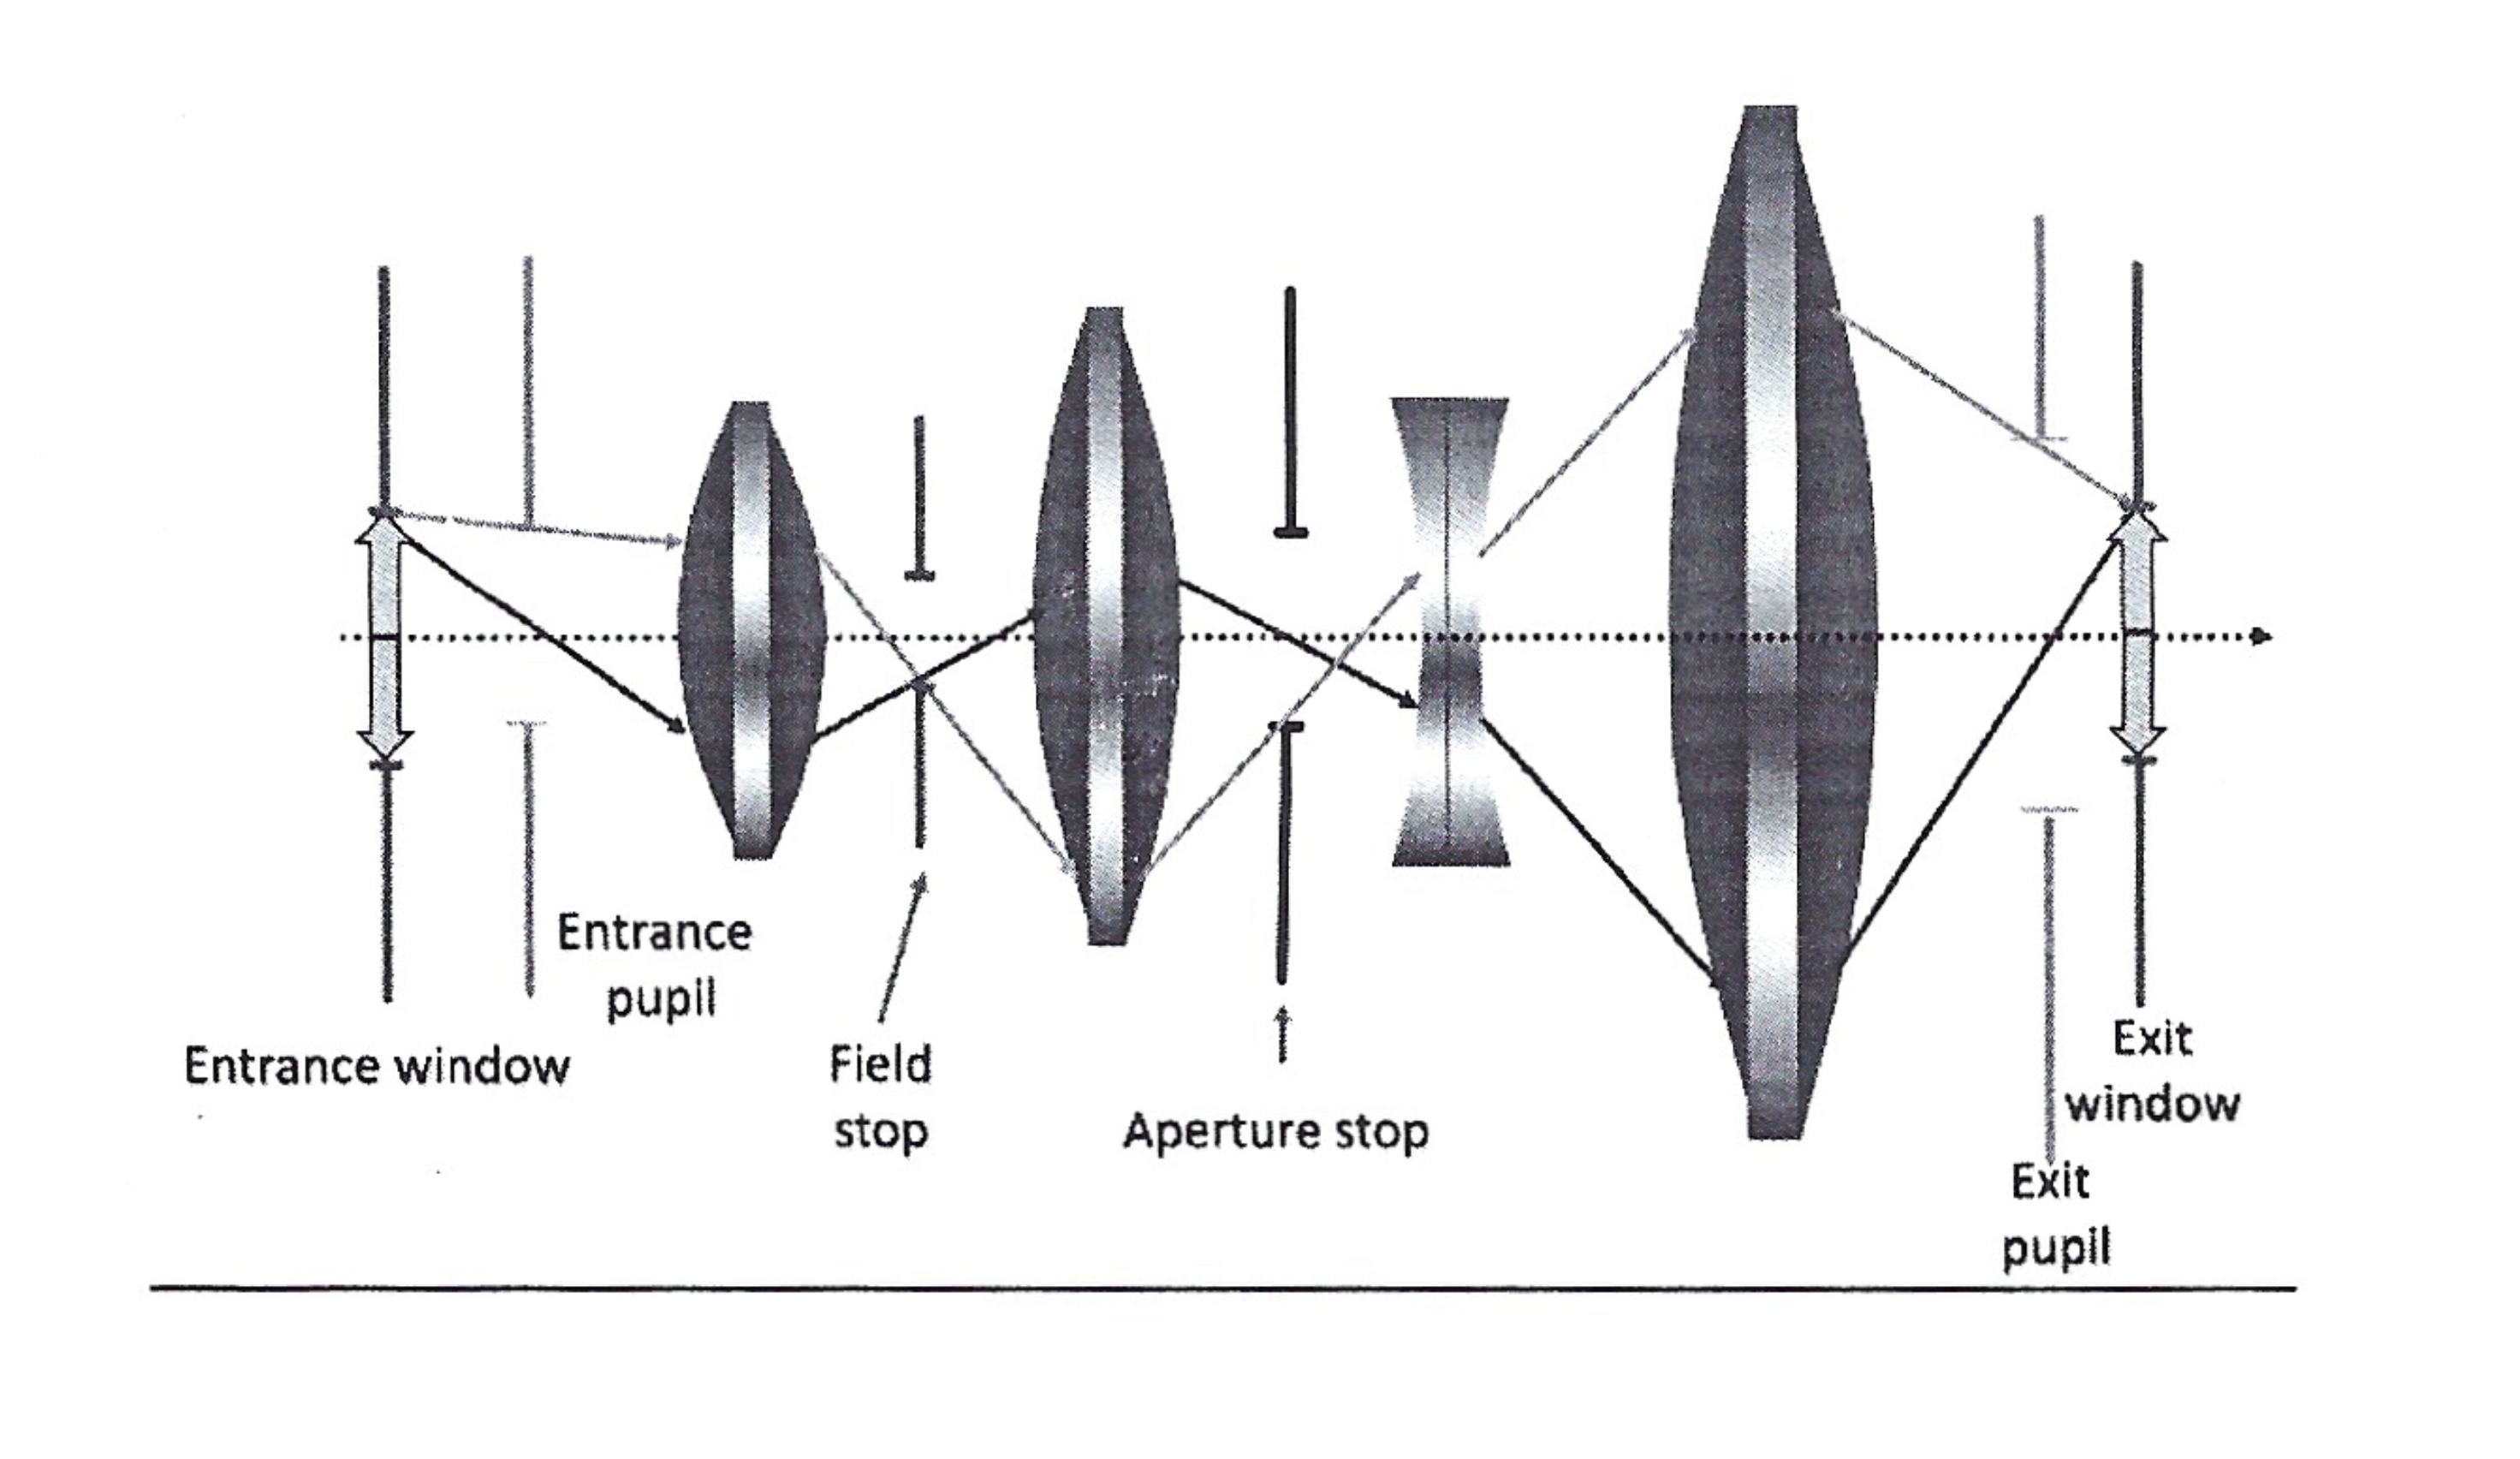
\includegraphics[width=4.0in]{figures/midterm/lens_system.png}}
\caption{Lens System}
\label{fig:m_1}
\end{figure}

% -----------------------------------------------------
% Sixth Problem
% -----------------------------------------------------

\item Find the resultant of \textbf{\underline{superposition}} of the wave E1 and E2 consider that: $E_1 = E_0 \hat{x} \cos (kz - \omega t)$, $E_2 = E_0 \hat{x}\cos(kz = \omega t)$. What does the the result represent? Give a practical example why this case could happen (trasmission line or optics). \textit{(3 points)}\\
 

% -----------------------------------------------------
% Seventh problem
% -----------------------------------------------------

\item Write the phasor of a plane waves of wavelength $\lambda$ and intensity $E_0$ which is propagating along the direction of wave vector $k_1$. Vector $k_1$ lies in the plane $xz$ and forms a 30 degree angle with respect to z. \textit{(4 points)}\\

% -----------------------------------------------------
% Eighth problem
% -----------------------------------------------------

\item An object of height $\SI{10}{C\metre}$ is placed $\SI{50}{c\metre}$ in front of a bi-convex lens with a focal length of $\SI{20}{c\metre}$. Which of the following is true about the image? \textit{(2 points)}\\

\begin{enumerate}[I]
  \item The image is virtual 
  \item The image is situated on the opposite side as the object
  \item The image is inverted
  \begin{enumerate}[A]
    \item I only
    \item I and II only
    \item II and III only
    \item II only
    \item III only
  \end{enumerate}
\end{enumerate}

% -----------------------------------------------------
% Ninth problem
% -----------------------------------------------------

\item Assume that the absolute values of the radii of curvature of the two surfaces of a thin lenses in air are $\SI{10.0}{c\metre}$ and $\SI{5.0}{c\metre}$ and that the index of refraction is 1.5. \textit{(4 points)}\\

\begin{enumerate}[a]
  \item What is the focal length of the lens if both surfaces are convex? 
  \item What is the focal length if one surface is convex and the other concave?
  \item What is the focal length if the lens is double-concave?
  \item Does it matter if we interchange the left and right surface?
\end{enumerate}

% -----------------------------------------------------
% Tenth problem
% -----------------------------------------------------

\item Find the \textbf{\underline{Poynting vector}} S and energy density field for the plane wave field $E = E_0\hat{x}\cos(kz-\omega t)$ traveling in vacuum. (Derive magnetic field first) \textit{(3 points)}\\

\end{enumerate}
\end{document}